\documentclass{beamer}
\usetheme{Madrid} % My favorite!
\usepackage{color}
\usepackage{hyperref}
\usecolortheme{orchid} % Simple and clean template
\setbeamercovered{invisible}
\setbeamertemplate{navigation symbols}{} 
\usepackage{natbib}
\usepackage{graphicx}
\usepackage{wrapfig}

%
\title[Improving meIRL-based motion modelling]{Improving meIRL-based motion modelling in video
games using general player classification}
\author[Inge Becht]{\large{Inge Becht}\\{\small Supervised by: Sander Bakkes}}
\institute[Universiteit van Amsterdam]
{\large Universiteit van Amsterdam}

\date{\today}
% \today will show current date. 
% Alternatively, you can specify a date.
%
\begin{document}
%
\begin{frame}
    \titlepage
\end{frame}

\begin{frame}
    \frametitle{Introduction}
    \begin{itemize}
        \item{Research topics in game AI}
            \begin{itemize}
                \item adaptive
                \item fair
                    \begin{itemize}
                        \item using imperfect information
                    \end{itemize}
            \end{itemize}
    \end{itemize}
    \begin{block}{Problem statement}
        To what extent can general player classification improve meIRL-based motion modelling
        in video-games?
    \end{block}
    \begin{itemize}
        \item Multiple aspects to this research
    \end{itemize}
\end{frame}
\begin{frame}
    \frametitle{Tools}
    \begin{minipage}[0.5\textheight]{\textwidth}
        \begin{columns}[T]
            \begin{column}{0.55\textwidth}
                \begin{itemize}
                    \item{Capture the Flag (CTF)}
                        \begin{itemize}
                            \item Team multi-agent environment
                            \item Straightforward game objective
                        \end{itemize}
                    \item{AISandbox}
                        \begin{itemize}
                            \item CTF AI development environment
                            \item Used for competitions
                        \end{itemize}
                    \item{Use existing AI}
                        \begin{itemize}
                            \item Terminator: 3$^{rd}$ place in competition
                            \item naive opponent response reasoner
                            \item adding of own motion modeller
                        \end{itemize}
                \end{itemize}
            \end{column}
            \begin{column}{1\textwidth}
                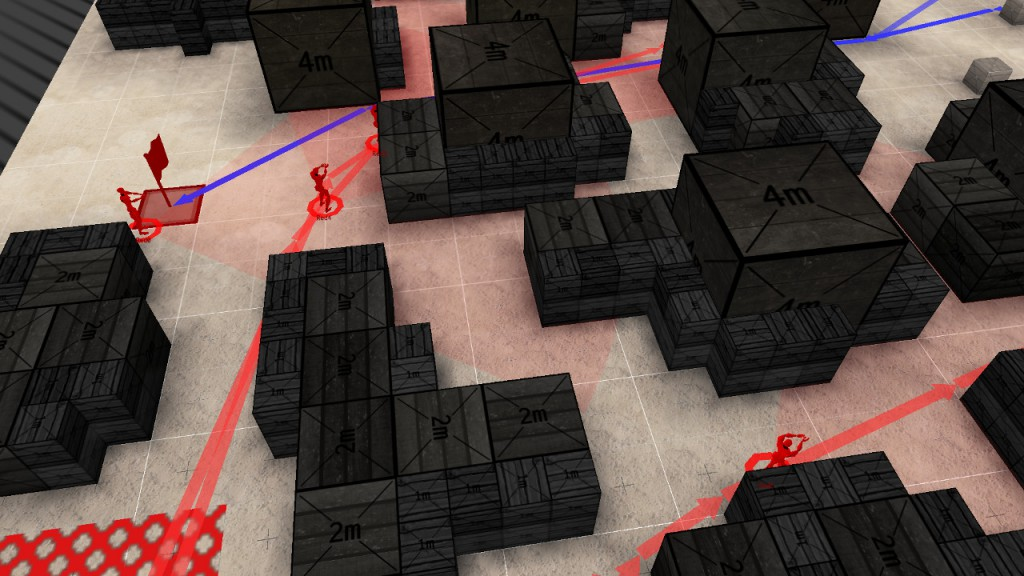
\includegraphics[width=6cm]{CTF_Sandbox.jpg}
            \end{column}
        \end{columns}
    \end{minipage}
\end{frame}

\begin{frame}
    \frametitle{Background Motion Modeling}
    \begin{minipage}[0.5\textheight]{\textwidth}
        \begin{columns}[T]
            \begin{column}{0.7\textwidth}
                \begin{itemize}
        \item Maximum Entropy Inverse Reinforcement Learning (meIRL)
            \begin{itemize}
                \item Position expressed in terms of features
                \item Construct reward function 
                \item Offline modelling
                \item Distribution grid
            \end{itemize}
        \item Has been done \citep{6374144}, but:
            \begin{itemize}
                \item No general modelling
                \item No examination of map invariance
                \item Different domain
                    \end {itemize}
                \item  General classes of specific behaviours
                \end{itemize}
            \end{column}
            \begin{column}{1\textwidth}
                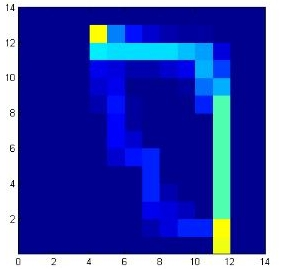
\includegraphics[width=4cm]{heat_map}
            \end{column}
        \end{columns}
    \end{minipage}
\end{frame}

        \begin{frame}
            \frametitle{Approach Player Classification}
            \begin{itemize}
                \item Prediction depends on classification
                \item Different behaviours, e.g.
                    \begin{itemize}
                        \item flag defensive
                        \item flag attacking
                        \item patrolling
                        \item flag running defender
                        \item flag retriever
                    \end{itemize}
                \item Classification Features,
                    \begin{itemize}
                        \item history of opponent spotting
                            \begin{itemize}
                                \item orientation
                                \item position (expressed in features)
                            \end{itemize}
                        \item game state, e.g.
                            \begin{itemize}
                                \item Both flags at base
                                \item Both flags gone
                                \item Enemy flag intercepted
                                \item Own flag intercepted
                            \end{itemize}
                    \end{itemize}
                \item Classification method not yet decided
            \end{itemize}
        \end{frame}

        \begin{frame}
            \frametitle{Approach Reasoner}
            \begin{itemize}
                \item Current Terminator motion model:
                    Only reasons on where enemy is seen
                \item Add enemy position prediction to Terminator 
                \item Further improvements:
                    \begin{itemize}
                        \item Ambushing enemy
                        \item Avoiding enemy
                        \item Anticipating actions
                    \end{itemize}
            \end{itemize}
        \end{frame}

        \begin{frame}
            \frametitle{Evaluation}
            \begin{block}{Problem statement (again)}
                To what extent can general player classification improve meIRL-based motion modelling
                in video-games?
            \end{block}
            \begin{itemize}
                \item How well can behaviour be classified?
                    \begin{itemize}
                        \item Needs labeled data to test with
                        \item Better than random
                    \end{itemize}
                \item Does general player classification successfully predict position?
                    \begin{itemize}
                        \item Absolute error comparison with \citep{6374144}
                    \end{itemize}
                    % Is this an honest measure of improvement?
                \item Improvement of Terminator?
                    \begin{itemize}
                        \item Create Competition
                        \item Compare performance by win-rate
                    \end{itemize}
            \end{itemize}
        \end{frame}

        \begin{frame}
            \frametitle{Plan}
            \begin{table}
                \centering
                \begin{tabular}{|l|p{5cm}|p{4cm}|}
                    \hline                        
                    Week No. & Research Planning & Report planning \\
                    \hline
                    \hline
                    18 &  Implement IRL motion model& \\
                    \hline
                    19 &  Implement IRL motion model& \\
                    \hline
                    20 &  Create classifier&\\
                    \hline
                    21 &  Implement into Terminator AI& \\
                    \hline
                    22 & & Preparation midpresentation and assignment 8\\
                    \hline
                    23 &  Evaluation of classifier, possible adaption&\\
                    \hline
                    24 &  Evaluation of AI performance & Assignment 9 \\
                    \hline
                    25 &  Finishing paper & \\
                    \hline
                    26 & Finishing paper & Preparing final presentation and logbook \\
                    \hline
                \end{tabular}
            \end{table}
        \end{frame}
        % End of slides

\bibliographystyle{apalike}
\begin{frame}
    \frametitle{References}
\bibliography{references}
\end{frame}
        \end{document} 
